\documentclass[10.5pt]{article}
\usepackage[a4paper,margin=2.1cm]{geometry}
\usepackage{amsmath,amssymb,booktabs,graphicx}
\title{Task 2b: which two-state plant? A proposal for decision}
\author{}
\date{3 November 2026 (numbers from \texttt{analysis/plant2\_check.py})}
\begin{document}
\maketitle
\vspace{-1.5em}
\section*{Criteria (CLAUDE.md) and how they were checked}
Open-loop unstable; low authority like the scalar case ($B=0.01$); controllable; equilibria with $u_{ss}\ne0$ that move with a
position setpoint $x_1=r$; the recoverable set inside the data box. All candidates use $B=(0,\,0.01)^\top$, the LQR weights
$Q=\mathrm{diag}(5,0.5)$, $R=0.1$ (gain from \texttt{scipy.linalg.solve\_discrete\_are}), and the actuator $|u|\le10$.
The recoverable set is the set of initial states from which the saturated LQR $u=\mathrm{clip}(-Kx,\pm10)$ reaches the origin
(161$\times$161 grid, 4000 steps). The safe band is the range of $g$ for which the closed-loop multiplier
$M=A-g\,BK$ (a model whose input slope is $\hat J_u=gB$ and whose state slope is right) has spectral radius below 1; it is
the two-state version of $(\hat J_x-1)/K<\hat J_u<(\hat J_x+1)/K$.

\begin{table}[h]\centering\footnotesize\setlength{\tabcolsep}{4pt}
\begin{tabular}{lcccc}
\toprule
 & scalar (current) & P1 & P2 & P3\\
\midrule
$A$ & $1.03$ & $\begin{bmatrix}1.02&0.05\\0&1.01\end{bmatrix}$ & $\begin{bmatrix}0.98&0.05\\0&1.03\end{bmatrix}$ & $\begin{bmatrix}1&0.1\\-0.05&1.01\end{bmatrix}$\\[8pt]
open-loop eigenvalues & 1.03 & 1.02, 1.01 & 0.98, 1.03 & $1.005\pm0.071i$\\
controllable & yes & yes & yes & yes\\
LQR gain $K$ & 10.29 & $(11.09,\ 11.90)$ & $(3.91,\ 10.38)$ & $(3.22,\ 10.37)$\\
closed-loop spectral radius & 0.927 & 0.956 & 0.954 & 0.956\\
equilibrium $x_2(r)$, $u_{ss}(r)$ & --, $-3r$ & $-0.4r$, $0.4r$ & $0.4r$, $-1.2r$ & $0$, $5r$\\
recoverable set (half-extent) & $|x|\le3.33$ & $|x_1|\le6.1$, $|x_2|\le4.7$ & $x_1$ unbounded, $|x_2|\le3.3$ & $|x_1|\le10.5$, $|x_2|\le7.6$\\
usable setpoints $|r|$ & $\le3$ & $\le6.1$ & $\le7.3$ & $\le1.8$\\
data box ($1.2\times$) & $|x|\le4$ & $|x_1|\le7.3$, $|x_2|\le5.6$ & $|x_1|\le8.8$, $|x_2|\le3.9$ & $|x_1|\le12.7$, $|x_2|\le9.2$\\
safe band $g$ & 0.29 -- 19.7 & 0.27 -- 17.3 & 0.15 -- 19.8 & 0.15 -- 19.7\\
spectral radius at $g=-1$ & 1.13 & 1.17 & 1.15 & 1.10\\
\bottomrule
\end{tabular}
\end{table}
\noindent For P2 the stable first state does not bound the recoverable set, so its data box is set by the setpoint range
(the equilibria of $|r|\le7.3$ need $|x_2|\le2.9$, $|u|\le8.8$).

\begin{figure}[h]\centering
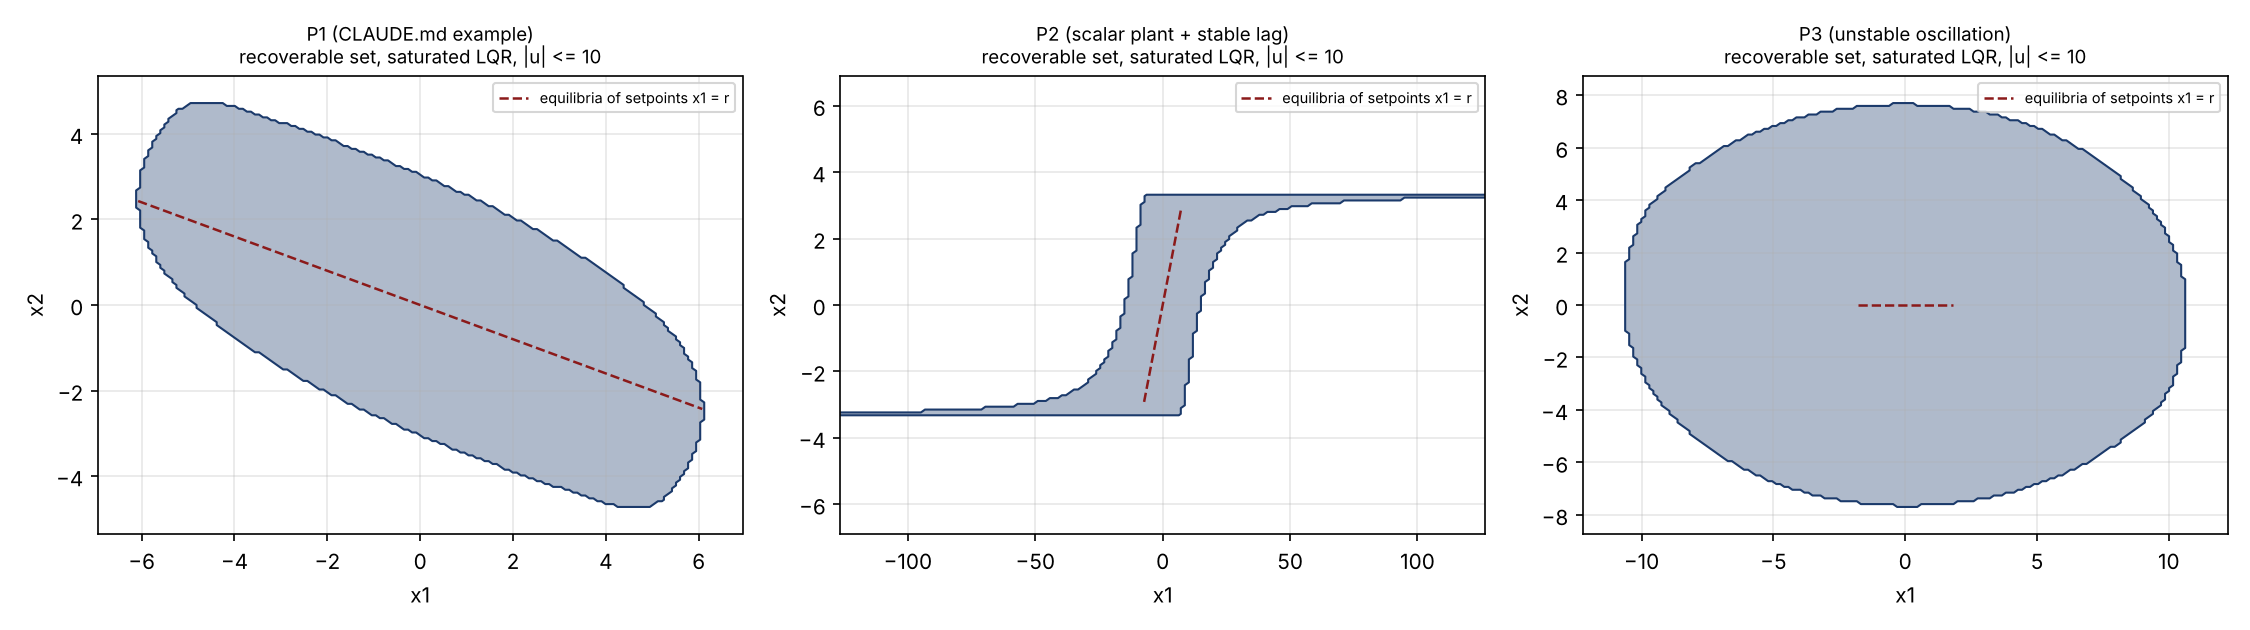
\includegraphics[width=\textwidth]{fig_recoverable.png}
\caption{Recoverable sets of the saturated LQR (shaded) and the equilibria of the position setpoints $x_1=r$ (dashed) for the
three candidates.}
\end{figure}

\section*{Assessment}
P1 (the CLAUDE.md example) meets every criterion. Both modes are unstable and coupled, the recoverable set is a genuinely
two-dimensional bounded region, the equilibria move along a line through the box ($x_2=-0.4r$, $u_{ss}=0.4r$), and the safe
band of the multiplier is close to the scalar one (0.27--17.3 $B$ against 0.29--19.7 $B$), so the same low-authority
sensitivity is present. Its only drawback is the small input per setpoint ($u_{ss}=0.4r$): the setpoint line crosses the
kink region at small $|u|$, which keeps the kink in play but means setpoints are mostly separated along $x$.

P2 nests the current study: its actuated, unstable state $x_2$ is exactly the scalar plant ($A=1.03$, $B=0.01$), and $x_1$ is a
stable lag that is the controlled output. Scalar results should carry over almost one to one, which makes it a clean
attribution test (does adding a state and a third surrogate input change the trap?) but a weak generality test: a reviewer
can say it is the same plant. It also adds a new error channel (the model may give $x_1^+$ a slope in $u$ that the true plant
does not have), which is interesting but not what Task 2b asks.

P3 is rejected: the setpoint equilibria all have $x_2=0$ and need $u_{ss}=5r$, so only $|r|\le1.8$ can be held, and the
oscillatory open loop complicates the landing window of $\Lambda^\star$.

\section*{Recommendation}
Use P1 as the second plant, as proposed in CLAUDE.md, with data box $|x_1|\le7.3$, $|x_2|\le5.6$, $|u|\le10$, setpoints
$r\in\{-4,-2,-1,-0.5,-0.25,0,0.25,0.5,1,2,4\}$ on $x_1$, starts on a $5\times5$ grid inside the recoverable set,
$Q=\mathrm{diag}(5,0.5)$, $R=0.1$, $Q_f=10Q$. Keep P2 as an optional control run if the P1 result differs from the scalar one
(it would say whether the difference comes from the plant's dynamics or from the two-state surrogate itself).

\section*{Cost}
Local work (me): the $n_x$-general versions listed in CLAUDE.md (plant, data, 3-input/2-output surrogate, 3-input label
estimator, ellipsoid kink metrics, vector DPC, DARE-based LQR study, matrix multiplier statistic), a CPU smoke test of every
milestone, and the short LaTeX note defining the matrix $\Lambda$ before it is used: about 3--4 working sessions.
Colab A100 (float64): Level 1, six families $\times$ 10 seeds, about 1 h (the label estimator in 3 inputs is the slow part);
DPC GRU and MLP through the 60 surrogates, 3 repeats, about 3--4 h; LQR study and $\Lambda^\star$ local (minutes to an hour).
Total about 5 h of A100 in two sessions (surrogates + oracle first, then the pre-registration, then DPC), as for Task 2a.

\section*{Addendum, 4 November 2026: the second error channel (P1a)}
Decision recorded: the user confirmed P1 with the settings above (docs/plant2/DECISION.md). The safe band above scales the
input slope only along $B$. A surrogate can also give $x_1^+$ a slope in $u$, which the true plant does not have. Write the
surrogate's input slope as $\hat J_u=0.01\,(h,\ g)^\top$ (true: $h=0$, $g=1$), keep the state slope correct
($\hat J_x=A$), and close the loop with the true LQR gain $K=(11.086,\ 11.903)$: the multiplier is $M(h,g)=A-\hat J_uK$.
Figure~\ref{fig:band2} maps its spectral radius (\texttt{analysis/plant2\_band.py}).

\begin{figure}[h]\centering
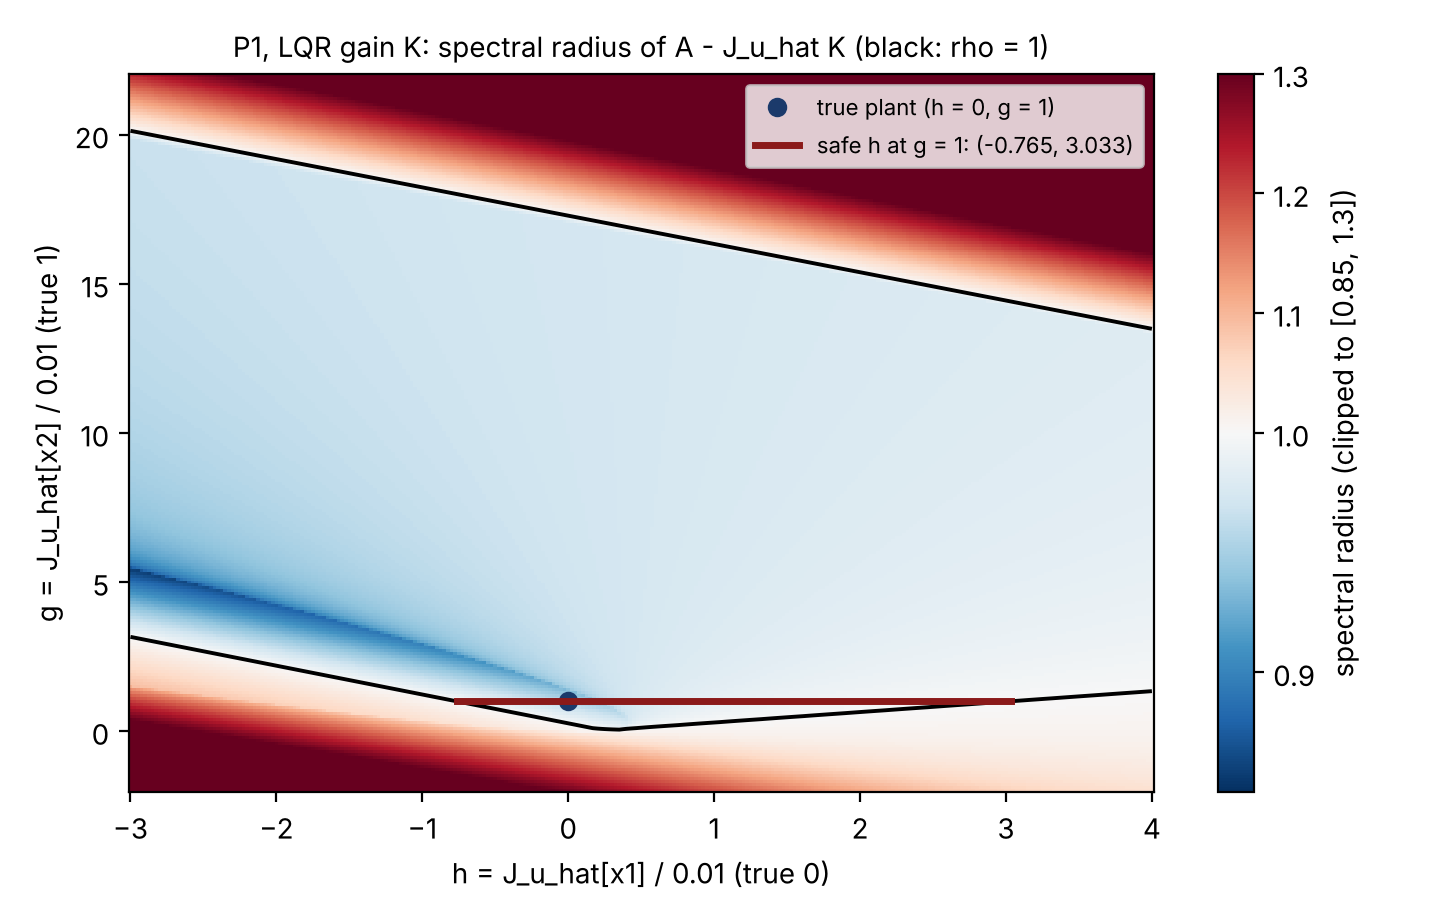
\includegraphics[width=0.82\textwidth]{fig_band2.png}
\caption{Spectral radius of $A-\hat J_uK$ for P1 at the LQR gain, as a function of the two input-slope entries
($h$ for $x_1$, $g$ for $x_2$, in units of 0.01). Black: $\rho=1$; inside the band the loop is stable. Dot: the true plant
($\rho=0.956$). Red: the safe range of $h$ at $g=1$.}
\label{fig:band2}
\end{figure}

\begin{table}[h]\centering\footnotesize
\begin{tabular}{lc}
\toprule
input slope for $x_2$, $g$ & safe range of $h$ (units of 0.01)\\
\midrule
0.29 & $-0.030$ to $1.008$\\
0.5 & $-0.248$ to $1.607$\\
1 (correct) & $-0.765$ to $3.033$\\
2 & $-1.800$ to $5.886$\\
5 & $-4.904$ to $12.950$\\
10 & $-10.08$ to $7.679$\\
17 & $-17.32$ to $0.300$\\
\bottomrule
\end{tabular}
\end{table}

\noindent Reading. With the $x_2$ input slope correct ($g=1$), the loop stays stable for $-0.77<h<3.03$, i.e.\ for a spurious
$x_1$ input slope between $-0.0077$ and $0.030$. The negative side is narrow: a wrong-direction slope of $0.77\,|B|$ into
$x_1$ is enough to destabilise the loop, even with every other slope exact. The band is asymmetric because $x_1$ is driven
through $x_2$ ($A_{12}=0.05>0$); a negative $h$ pushes $x_1$ against the way the controller moves it. Near both edges of the
$g$-band the safe range of $h$ shrinks to almost nothing (at $g=0.29$: $-0.03$ to $1.0$; at $g=17$: up to $0.30$). Check: at
$h=0$ the $g$-band is $0.261$ to $17.29$ (written $0.27$ to $17.3$ in the table above, rounding).
Consequence for the study. The kink errors of the scalar surrogates were $6.7$ to $201\,B$ at the peak, so a two-state
surrogate's $x_1$-column input slope only needs a small fraction of that to leave the band. The Level 1 metrics and the LQR
analysis of P1 will therefore report both input-slope entries separately (peak $|\hat J_u[x_1]|/|B|$ and
$|\hat J_u[x_2]/B-1|$), and the closed-loop multiplier is computed with the full $2\times1$ $\hat J_u$, as
\texttt{plant2\_core} already does.

\end{document}
